\chapter{Security}

Dal momento che i dati che trattiamo e ricaviamo dall'analisi hanno rilevanza conoscitiva e valore in termini di mercato e ricerca, risulta fondamentale considerare un ambiente sicuro in cui accogliere tali informazioni. Tale perimetro deve però garantire, contemporaneamente alla discrezione relativamente all'accesso del dato, un livello sufficiente di astrazione dalla generica interazione esterna, permettendo un massimo controllo sull'interezza del sistema.

\begin{figure}
	\centering
	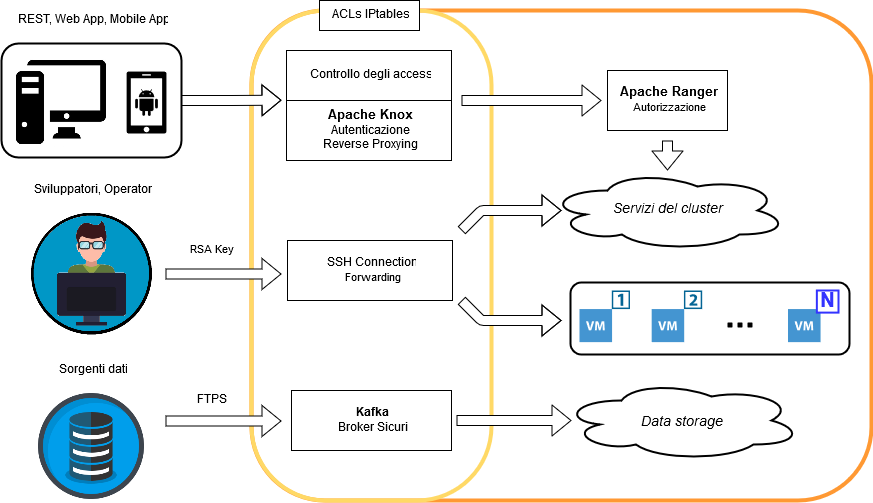
\includegraphics[scale=0.4]{Figures/security_diagram.png}
	\decoRule
	\caption[Infrastructural Stack]{Struttura del perimetro di sicurezza}
	\label{fig:security_diagram}
\end{figure}
La struttura progettata risulta, dunque, articolata su due livelli:
\begin{itemize}
	\item frontend, che si occupa dell'interazione dell'utente con i servizi forniti dal cluster;
	\item cluster, ossia i nodi sottostanti, che garantiscono un livello di sicurezza più specifico per ogni servizio interpellato.
\end{itemize}
Il primo problema da porsi nello sviluppo di una struttura di sicurezza risulta essere la definizione delle entità che possono interagire con il sistema e in quale misura tali interazioni avvengono, in modo da fornire una soluzione adatta sia in termini di confidenzialità per le parti che per facilità d'uso.
\newline
Parliamo, quindi, di:
\begin{itemize}
	\item operatori tecnici: sviluppatori o amministratori del sistema, che necessitano di accessi più profondi e possono lavorare all'interno della rete aziendale.
	\item utenti esterni: clienti o personale generico, che necessitano di utilizzare i servizi del cluster, senza possibilità di modificarne la struttura.
	\item sorgenti dati: data streams esterni, inviano dati su cui si lavorerà con gli strumenti presenti nel cluster.
\end{itemize}
Per ciascun utente si sono considerati approcci differenti, commisurati alle esigenze. 
Le richieste avvengono su un ristretto numero di porte abilitate alla comunicazione con l'esterno e viaggiano su canali sicuri, tramite l'utilizzo di protocolli quali HTTPS, SSH e FTPS.
\newline
In un secondo momento le chiamate vengono autenticate tramite provider dedicati come LDAP o Kerberos, per poi essere sottoposte ad un controllo di autorizzazione, atto a verificare che la richiesta sia congrua ai diritti dell'utente.
\newline
L'esito di ciascun passaggio viene registrato da un servizio di auditing, che permette di tenere traccia delle richieste e degli accessi al sistema, in modo da identificare eventuali abusi o tentativi di forzatura del sistema.

\pagebreak

\section{Knox}

Apache Knox è un Application Gateway, componente della suite di strumenti Hadoop, che fornisce varie funzionalità in termini di sicurezza per clusters Hadoop, specialmente se coadiuvato da altri elementi.
\newline
Nella struttura in esame riveste il ruolo fondamentale di "Reverse Proxying" dei servizi offerti dal cluster e di autenticazione e "Access Control".
\subsection{Reverse Proxying}
Il gateway Knox fornisce un servizio di mascheramento che permette di definire un URL da mostrare all'utente esterno corrispondente a ciascuna chiamata rivolta al cluster. In questo modo è possibile distinguere interfaccia e implementazione del servizio, mantenendo confidenziale la struttura dell'architettura sottostante e garantendo la modularità del sistema.
\newline
Ogni servizio che necessiti di Knox deve essere dichiarato all'interno di uno specifico file di topologia. La topologia è un file XML che dichiara le componenti associate a Knox, quali provider di autenticazione e autorizzazione, e i servizi gestiti dal file in esame.
A questo vengono accompagnati due file di definizione del servizio:
\begin{itemize}
	\item service.xml, che definisce la struttura della chiamata che verrà associata al servizio interessato;
	\item rewrite.xml, che definisce tramite regex la politica di riscrittura che deve essere seguita, prima che la chiamata venga inoltrata al cluster.
\end{itemize}
Le chiamate che possono essere fatte tramite Knox seguono i dettami del protocollo REST, riportando indirizzo, topologia e servizio richiesto nell'URL sottoposto.
% procedimento di reverse proxying ???
\pagebreak

\subsection{Autenticazione e Access Control}
Il gateway Knox si presenta come unico access point sicuro per le interazioni con il cluster, che siano esse tramite API REST che attraverso chiamate HTTP/HTTPS. Ogni richiesta viene inoltrata previa sottomissione di credenziali. Queste vengono autenticate da Knox tramite il provider dichiarato dalla topologia selezionata, LDAP o Kerberos.
Successivamente la chiamata autenticata viene sottoposta all'entità specificata per l'autorizzazione che garantisce controllo sugli accessi ai servizi del sistema.
Infine, una volta garantita la bontà della richiesta, viene sottoposta al servizio per l'esecuzione.
\pagebreak

\section{Ranger}

Apache Ranger \cite{ranger_doc} è un framework che si occupa di definire e gestire la sicurezza del dato all'interno di un cluster Hadoop. Questo avviene tramite l'utilizzo di un sistema di autorizzazione specifico per ogni servizio presente nel cluster che centralizza le logiche di autorizzazione per le varie risorse del sistema. La gestione di Ranger può avvenire sia tramite interfaccia grafica web, sia tramite chiamate REST al nodo su cui risiede il framework. Infine, garantisce una profonda conoscenza per quanto riguarda le interazioni con il cluster, tramite un servizio di audit che osserva le operazioni effettuate in tempo reale e le registra su HDFS o Solr.
\newline

\subsection{Autorizzazione}

Nel momento in cui una richiesta a un servizio del cluster viene autenticata dal provider scelto, deve essere sottoposta al controllo di Ranger, per verificare i privilegi dell'utente nei confronti della risorsa richiesta. È possibile gestire il processo di autorizzazione su due livelli differenti: discriminando rispetto caratteristiche di chi effettua l'accesso o a che unità di lavoro appartiene (access authorization) o relativamente alla risorsa richiesta (resource authorization).
\newline 
All'interno di tali approcci possiamo riconoscere ulteriori distinzioni. Relativamente al controllo degli accessi degli utenti:
\begin{itemize}
	\item Role based (RBAC), che valuta l'accesso in base a criteri di ruolo e privilegi dell'utente;
	\item Attribute based (ABAC), una specializzazione del RBAC, che considera nella valutazione anche attributi aggiuntivi, come indirizzo IP, luogo di login o dati dell'utente.
\end{itemize}
Per quanto riguarda,invece, l'accesso alle risorse, essendo un framework rivolto all'utilizzo in un ambiente Hadoop, Ranger mette a disposizione alcuni plugin per interagire direttamente con i principali servizi presenti nella suite, garantendo un controllo più specifico e profondo riguardo quali operazioni l'utente possa e non possa fare. I plugin sono programmi in Java incapsulati in processi del servizio di riferimento che si occupano di caricare le regole da un server centrale e memorizzarle localmente in un file. Tra i servizi riconosciuti troviamo:
\begin{itemize}
	\item HDFS
	\item HBase
	\item Hive
	\item Yarn
\end{itemize}
Ad esempio, per quanto riguarda Hive, le regole di autorizzazione permettono di specificare per ogni regola quali operatori è possibile utilizzare nelle query al database, chi può effettuarle e a quali campi può avere accesso.
%immagine policy
\newline

\subsection{Regole "Tag Based" e persistenza dei dati}

Versioni più recenti di Ranger hanno introdotto la possibilità di utilizzare regole di sicurezza basate su etichette. Queste vengono attribuite a varie risorse dai vari servizi in modo da definire lo stesso tipo di regola per entità differenti senza doverlo definire esplicitamente, rendendo più semplice le operazioni di controllo degli accessi e di gestione delle risorse. Le etichette e la loro definizione sono tenute in un "Tag Store", mentre un processo di sincronizzazione TagSync si occupa di mantenere le informazioni sempre aggiornate tra i servizi che ne fanno uso.
\newline
Tutte i dati relativi alla logica di sicurezza sono memorizzati in locale, in uno database MySQL su uno degli hosts, che mantiene tutte le informazioni relative a regole e utenti previsti dal framework. La coerenza del sistema viene garntita da un processo di sincronizzazione dedicato che aggiorna le liste di utenti, gruppi e ruoli con LDAP/Active Directory e le opzioni di configurazione con Ambari.
\newline